\begin{section}{Preface}
The preceding sections have been devoted to a development of various methodologies for ab initio intermolecular force
field development, all generally assuming that \acrfull{sapt} can be used as a benchmark electronic structure
theory. Critically, and especially given the developments discussed in \chref{ch:anisotropy},
we can now usually expect our model force field energies to be within
\kjmol{\textasciitilde1} of the \sapt reference values! In spite of this
success, we note that high precision between the model
and \sapt can only lead to improved molecular simulation provided that the \sapt energies \emph{themselves} are
accurate, either with respect to the exact underlying \acrfull{pes} or (for practical
purposes) with respect to gold-standard \ccsdt calculations. Indeed, if \sapt
and \ccsdt differ by several \kjmol{}, there is little point in developing
\sapt-based force fields with \kjmol{<1} accuracy! This raises to two
fundamentally important questions regarding our methodology for force field
development. First, for what types of systems might we expect \sapt to be inaccurate? Secondly,
for such systems where \sapt does not achieve a desired level of accuracy, how
must we modify our typical methodology for ab-initio force field development?

The above questions have been addressed, in part, by myself and other
researchers. Errors in \sapt are often greatest for
hydrogen-bonded\cite{Parker2014a} or extremely ionic systems,

The overall purpose of this chapter is to address, in part, the above
concerns. 

Nevertheless (and as discussed in \chref{ch:anisotropy} and below),
significant \sapt 

\end{section}
\begin{section}{Introduction}


What, however, should be done for systems where \acrshort{sapt} itself
is in significant error?\cite{Parker2014a} 

Back in 2013, at the start of this project, we encountered a series of systems
for which \sapt did indeed seem to be breaking down.


    %%%%%%%%%%%% SAPT Breakdown %%%%%%%%%%%%%%%
    \begin{figure}
    \centering
    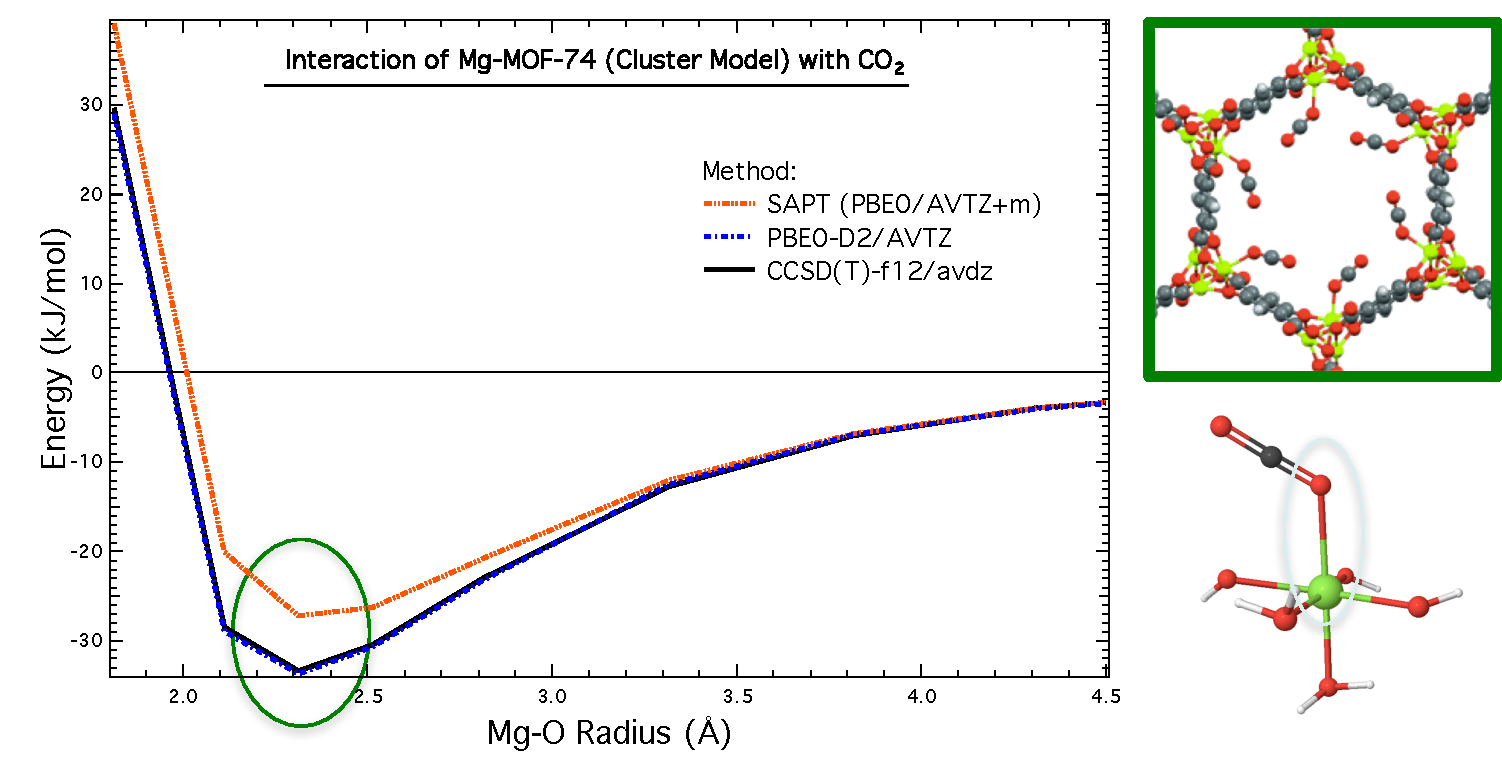
\includegraphics[width=1.0\textwidth]{lmoeda/sapt_breakdown.pdf}
    \caption{
Model \pes for interactions between \co and \mgmof.  (Left) Interaction
energies between \co and a cluster model of \mgmof (shown bottom right),
computed at a \ccsdtf (black), \sapt (orange), and/or \pbeod (blue) level of
theory. Discrepancies
between \sapt and \ccsdtf in the minimum-energy region of the potential have
been highlighted. (Top right)
The structure of \co-bound \mgmof. (Bottom right) The structure of the cluster
model used for \mgmof, where the circled atom pair indicates the relevant Mg-O
radius from the x-axis in the leftmost figure.
            }
    \label{fig:rmse}
    \end{figure}
    %%%%%%%%%%%% SAPT Breakdown %%%%%%%%%%%%%%%

\end{section}{Introduction}


=======================

\gls{sapt}
\gls{saptg}
\gls{abintff}


